\documentclass[xcolor=dvipsnames]{beamer} 
\usetheme{Boadilla}
%\usecolortheme[named=Blue]{structure}
\usepackage{times}
\usepackage{color}
\usepackage{graphics}
\usepackage{epsfig}
\usepackage{hyperref}
\usepackage{beamerthemesplit}


\title{Learning from the Statistician's Lab Notebook}
\author{Deborah Nolan \& \\ Duncan Temple Lang}
\date{July 12, 2010}
\begin{document}

\maketitle
\parindent=0pt

\begin{frame}\frametitle{Outline}
\begin{itemize}
\item Motivation - Methodology Meets Context 
  
  \medskip
  
\item Lab Notebook as an Interactive, Dynamic Document Database
  \medskip
  
  \item Examples - Geolocation \& Election Anomalies
    \medskip
    
\item Infrastructure - XML, R
\medskip
\item Next Steps 

\end{itemize}
\end{frame}


\begin{frame}\frametitle{Motivation}

\begin{itemize}
\item Focus on statistical experience, reasoning and applications
  \textit{throughout} statistical training (Brown \& Kass, \textit{TAS} 2009);
  \medskip
  
  \item Biggest holes in our educational fabric, limiting the ability of graduates to apply statistics, occur where methodology meets context (Wild, \textit{ISIR}, 2007)
  \medskip
  
  \item Change the culture of statistics training to engage students in
  active, participatory ``effortful learning'' in addition to critical
  study (Nolan \& Temple Lang, \textit{TAS}, 2010);
  
\end{itemize}
\end{frame}

\begin{frame}\frametitle{Where Do Students Encounter Statistical Experience?}
\begin{itemize}
\item �Let them do projects.�  (Wild \& Pfannkuch, \textit{ISIR} 1999)
\item Capstone course
\item Case Studies
\end{itemize} 

\begin{block}{US NRC, 1996}
Inquiry is a multifaceted activity that involves:

\begin{columns}
 \begin{column}{0.45\textwidth}
 \begin{itemize}
  \item making observations
    \item posing questions
  \item examining other sources  to see what is already known
   \item reviewing what is  known in light of experimental evidence
  
 \end{itemize} 
\end{column}

  \begin{column}{0.45\textwidth}
 \begin{itemize}
    \item planning investigations
  \item using tools to gather, analyze, and interpret data
  \item proposing answers, explanations, and predictions 
  \item  communicating results
 \end{itemize} 
\end{column}
\end{columns}
 
\end{block}


\end{frame}


\begin{frame}\frametitle{Explorations in Statistics Research}

\begin{columns}
 \begin{column}{0.45\textwidth}
\begin{tabular}{ccl}
\multicolumn{2}{c}
{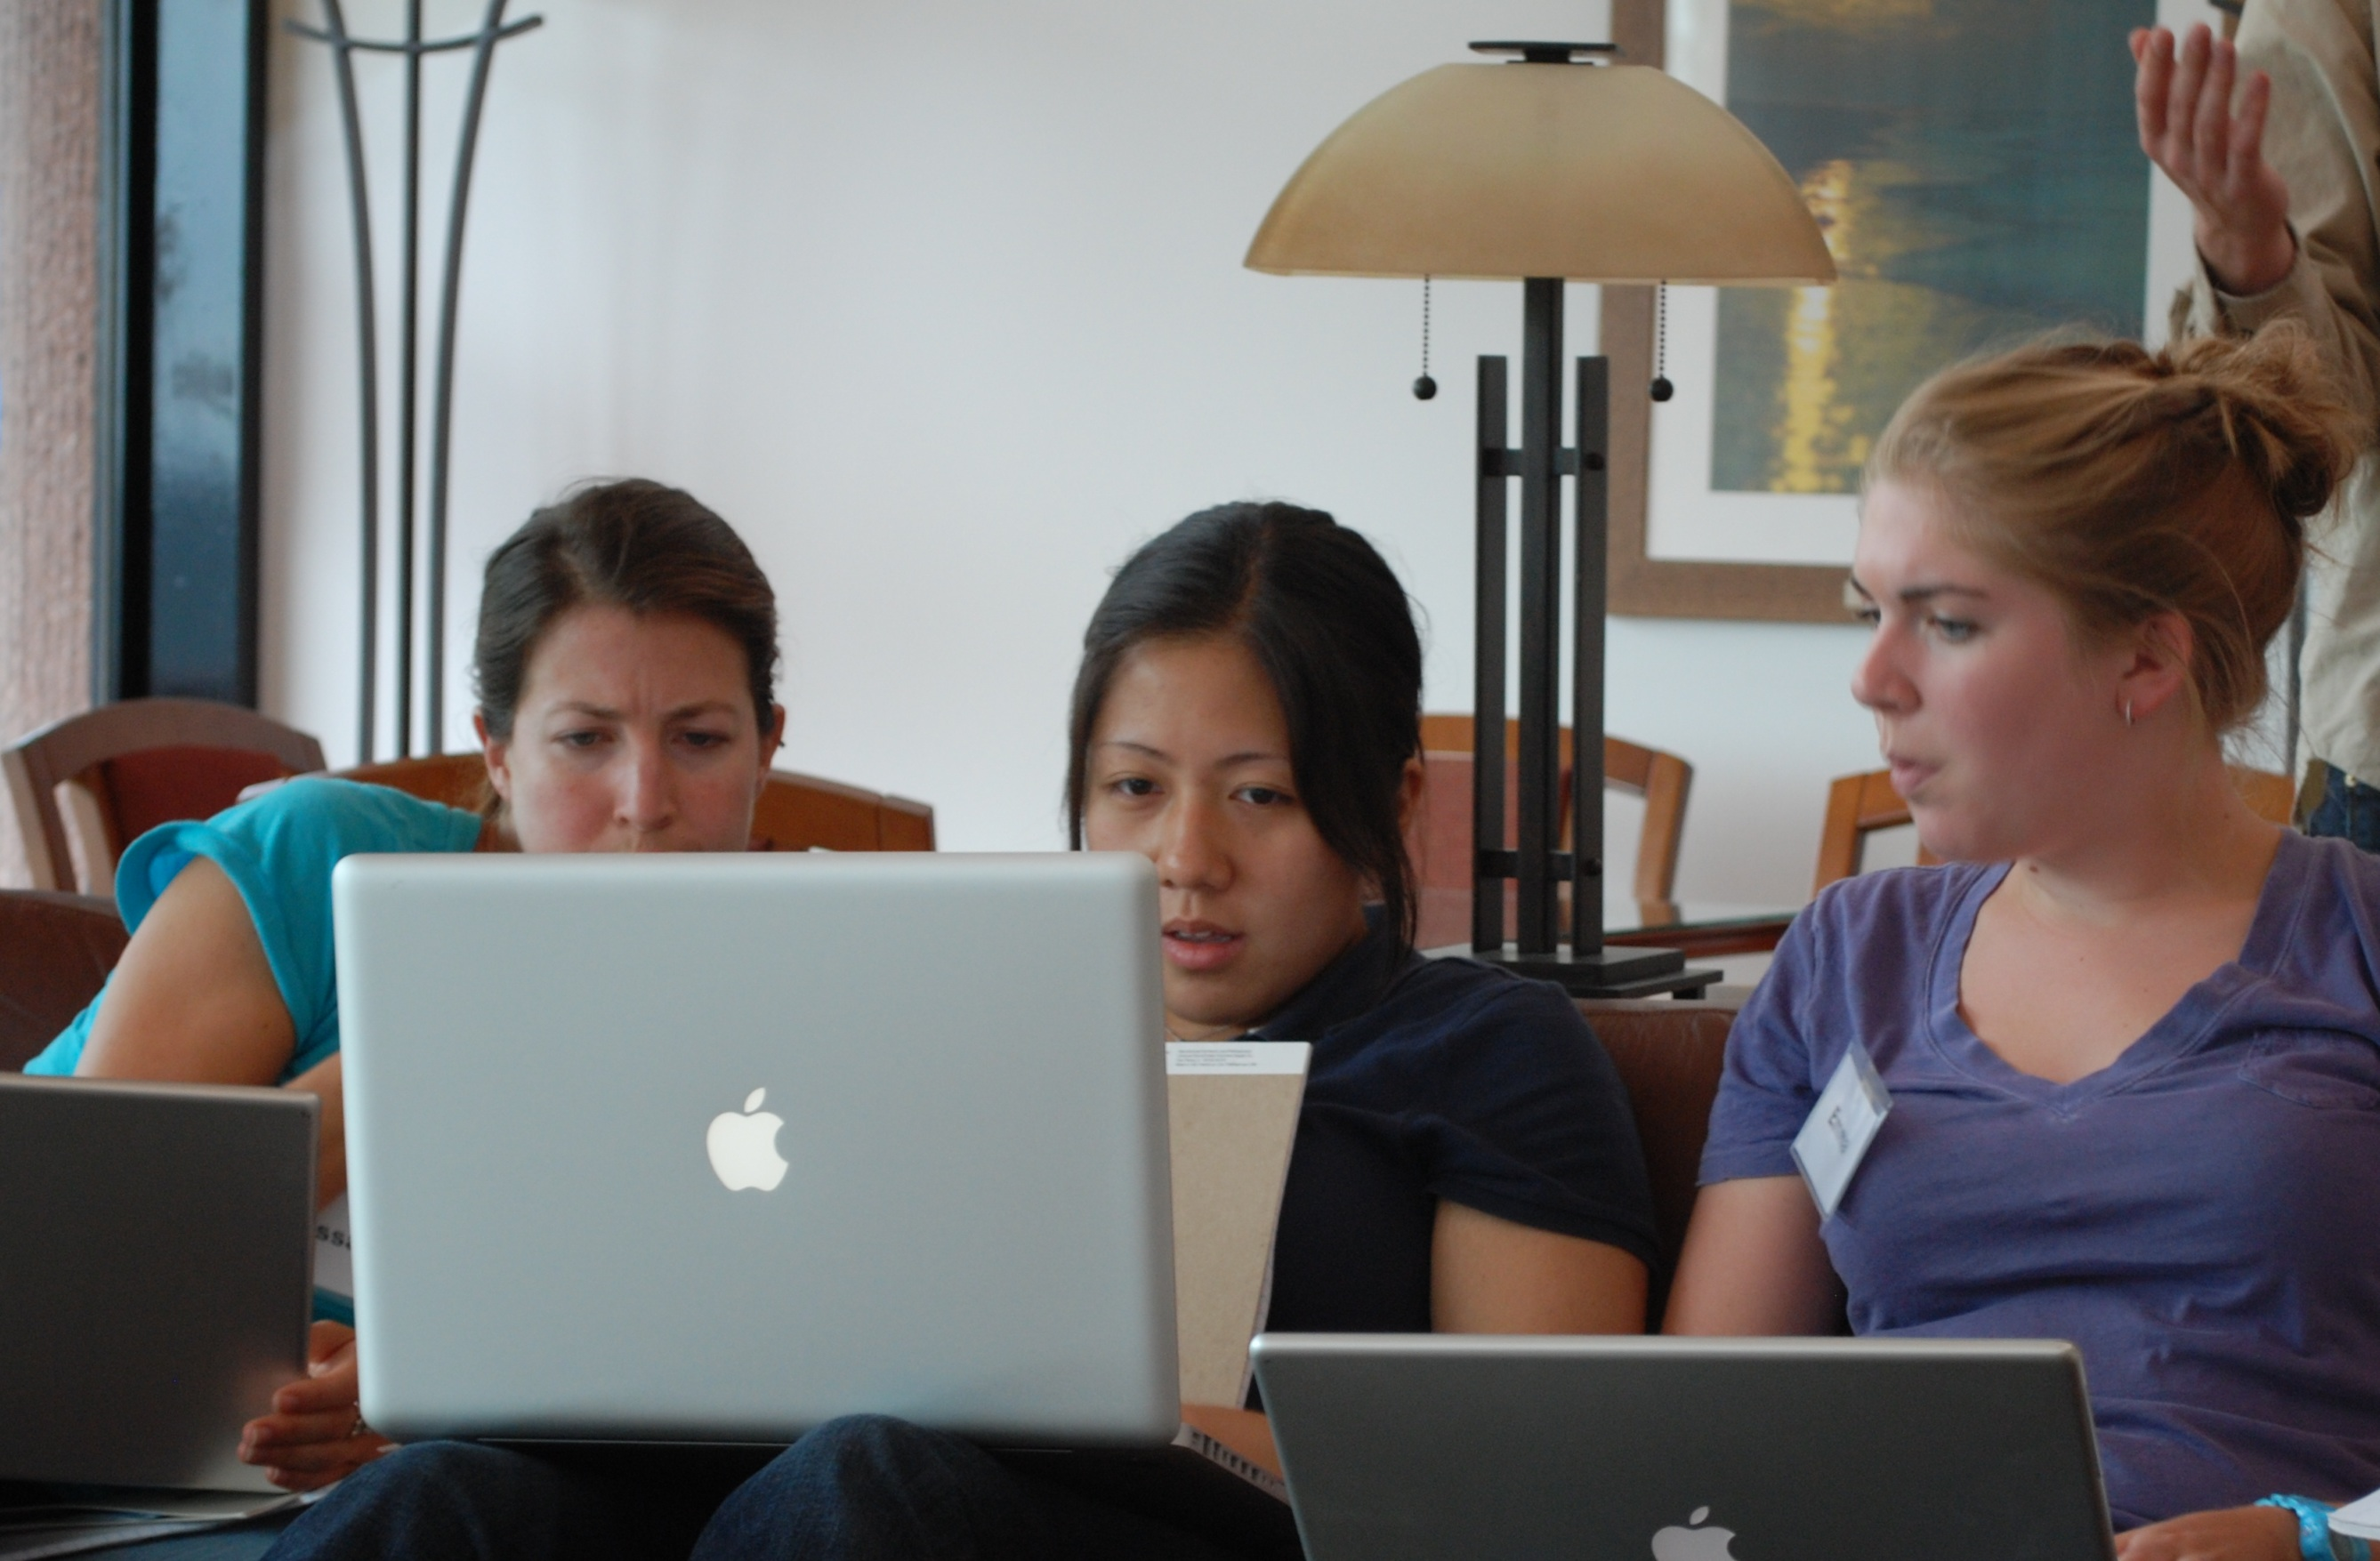
\includegraphics[width=2in]{images/StudentWork.jpg}}\\
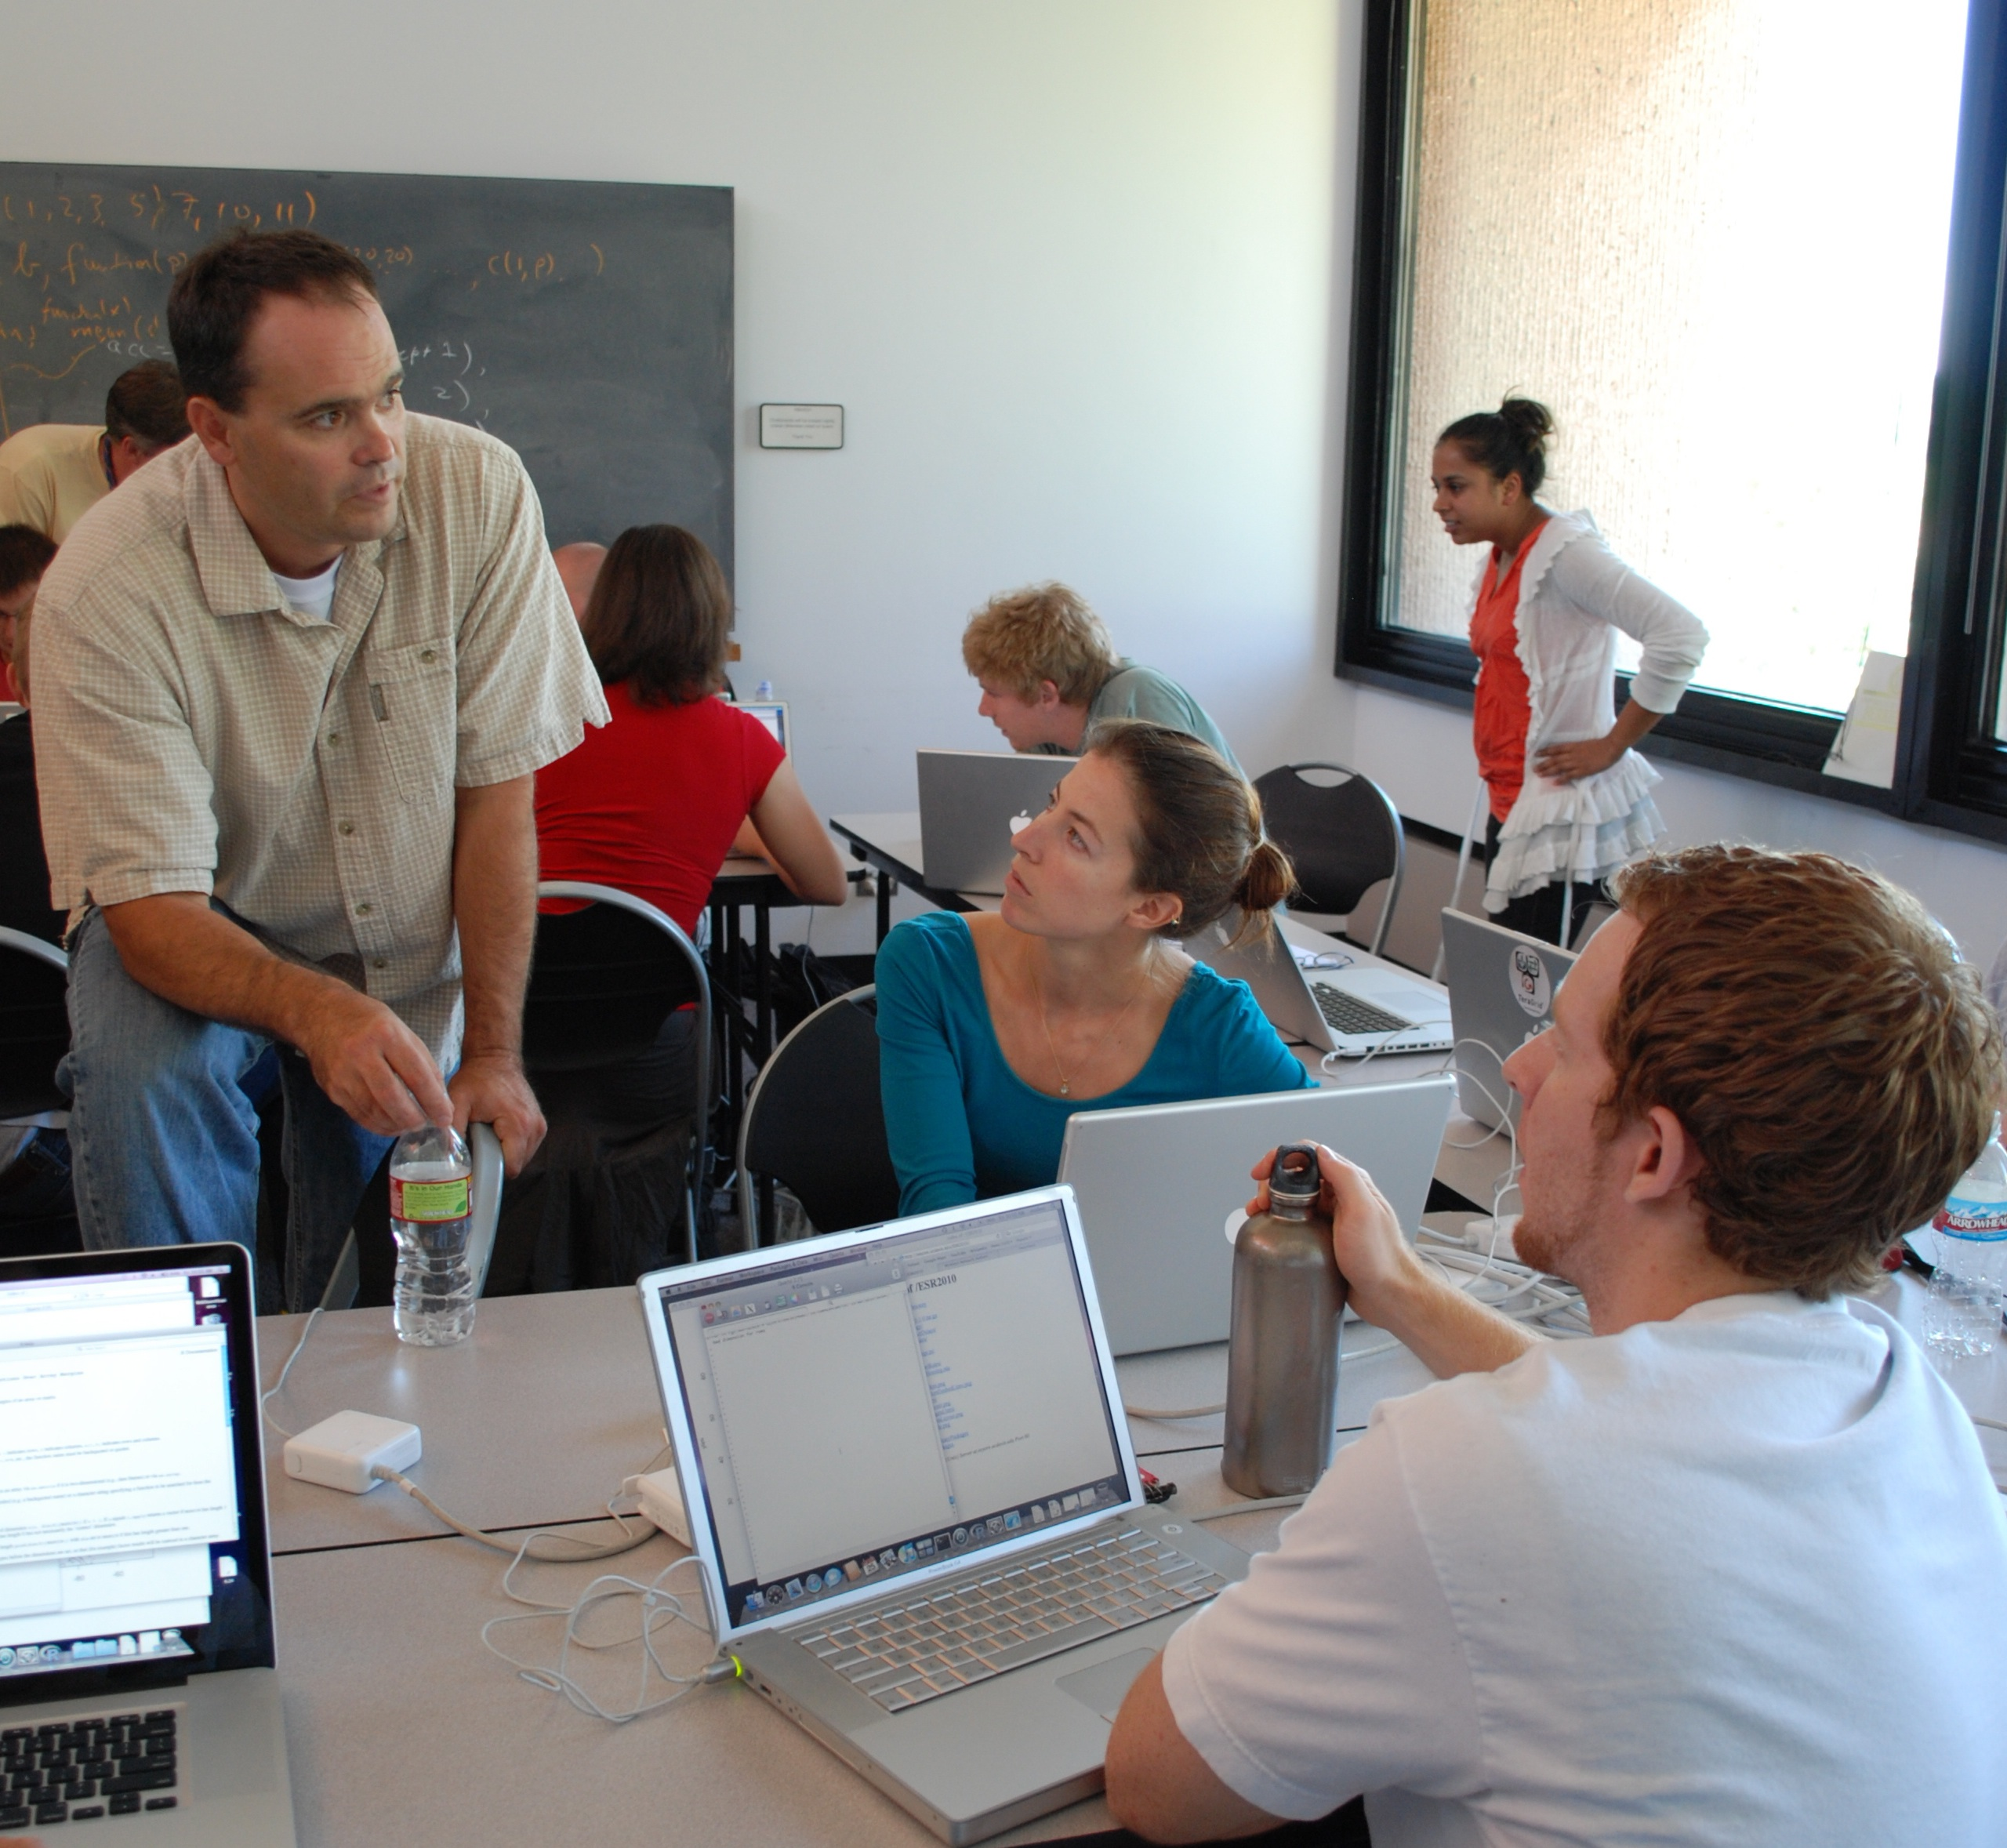
\includegraphics[width=1in]{images/ExpertDiscuss.jpg} &
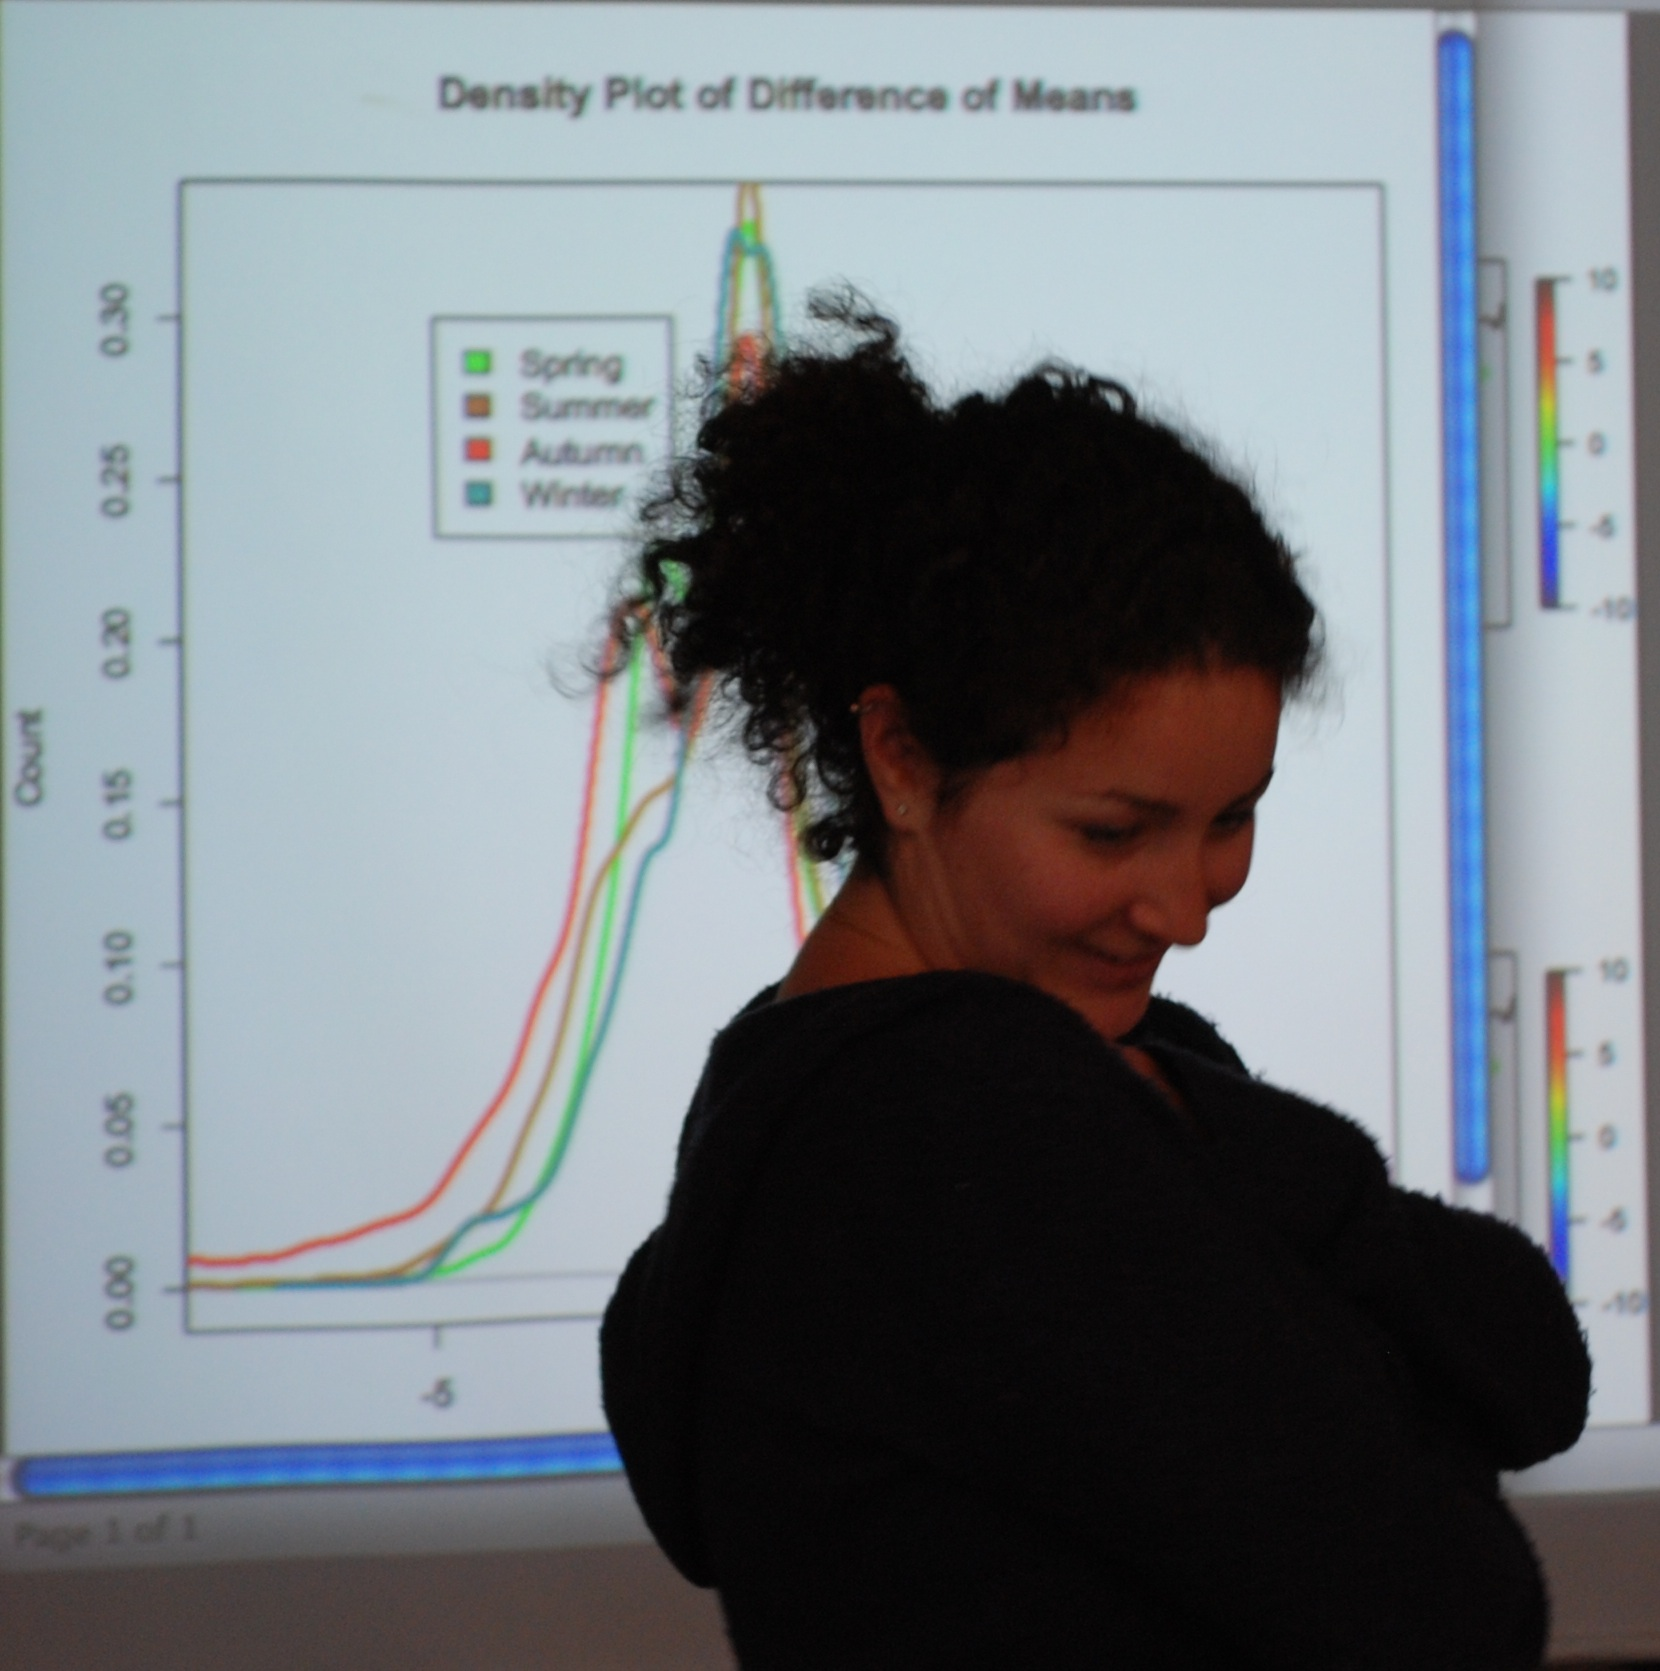
\includegraphics[width=1in]{images/StudentPresent2.jpg} \\
\end{tabular}
\end{column}
 
 \begin{column}{0.45\textwidth}
 The seven day workshop
 is designed so that students get a sense of how statisticians approach large, complex problems. 
 
 \bigskip
 
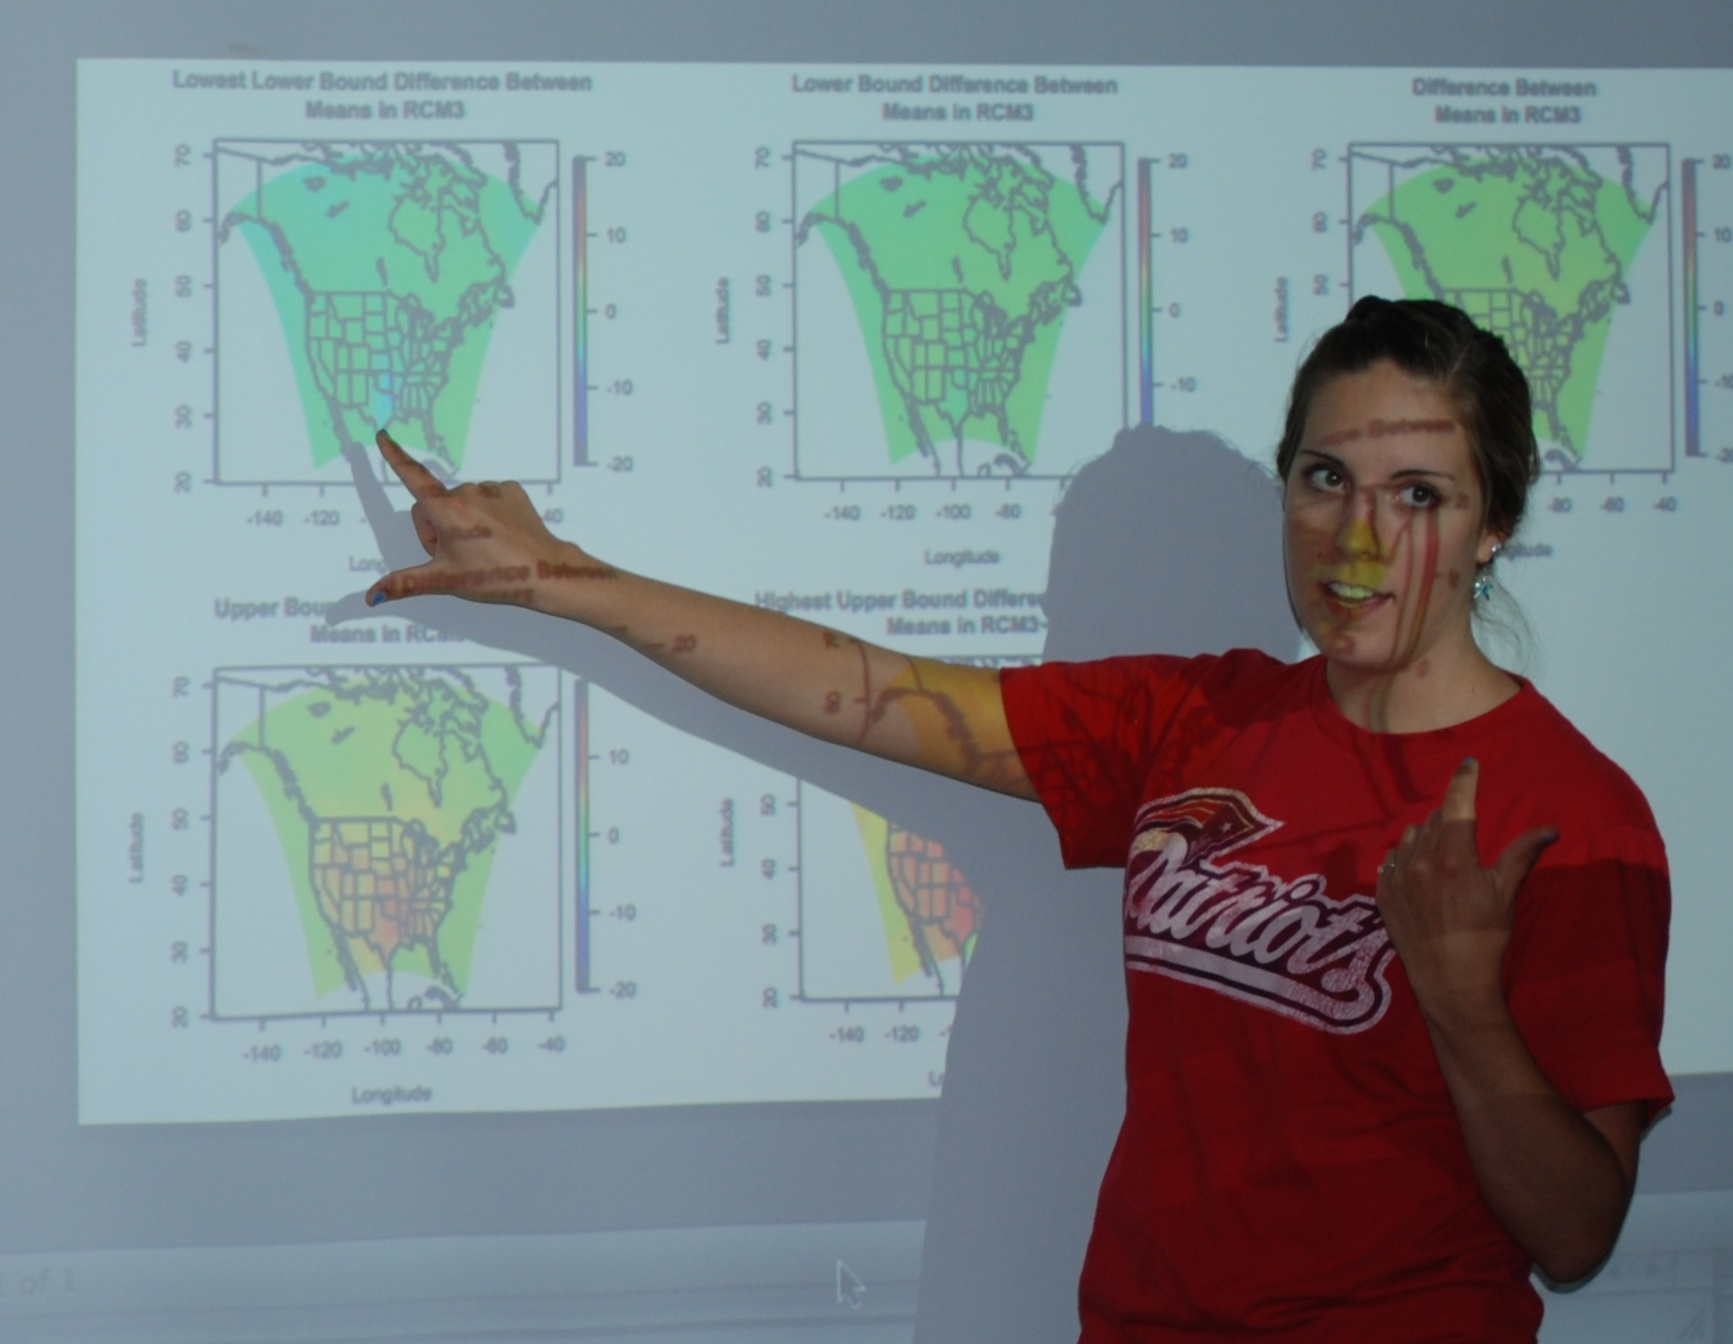
\includegraphics[width=1.5in]{images/StudentPresent.jpg} 

\end{column}
\end{columns}
\end{frame}

\begin{frame}\frametitle{Educational Materials}

\begin{itemize}
\item \textit{Statistics: A Guide to the Unknown}, (2006) Peck et al
\medskip
\item JSE Data Archive \texttt{www.amstat.org/publications/jse}
\medskip
\item Rice Virtual Lab in Statistics \texttt{onlinestatbook.com/rvls.html}
\medskip
\item CAUSEweb.org Resources \texttt{www.causeweb.org/cwis}
\medskip
\item Stat Labs \texttt{www.stat.berkeley.edu/users/statlabs}
\medskip
\end{itemize}

\end{frame}

\begin{frame}\frametitle{Data Analysis Process}

\begin{itemize}
\item decompose the problem 
\item identify key components
\item  abstract and formulate different strategies 
\item connect the original problem to the statistical framework
\item choose and apply methods 
\item reconcile the limitations of the solution
\item communicate findings
\end{itemize}
\end{frame}


\begin{frame}\frametitle{Electronic Lab Notebook}
\begin{itemize}
\item Capture computations, analyses, notes, and thought process 

\medskip

\item Reproduce findings for yourself and others 

\medskip

\item  Store database of all the activities within the data analysis

\medskip

\item  Project different views for different audiences, e.g.
\begin{itemize}
\item paper for a journal
\item technical report with more extensive details
\item  interactive document to drill down and explore at different levels of detail
\end{itemize}
\end{itemize}
\end{frame}

\begin{frame}\frametitle{Electronic Lab Notebook}

Notebook as a Teaching/Learning Medium

\begin{itemize}
\item Control complexity and other environmental settings
\item Provide multiple pathways to explore
\item Focus attention on what is new and accelerate through what has already been mastered
\item Allow students to efficiently �unlock the stories in data�
\item Encourage students to �just try things out�
\end{itemize}
\end{frame}

\begin{frame}  \frametitle{The Document as a Database}
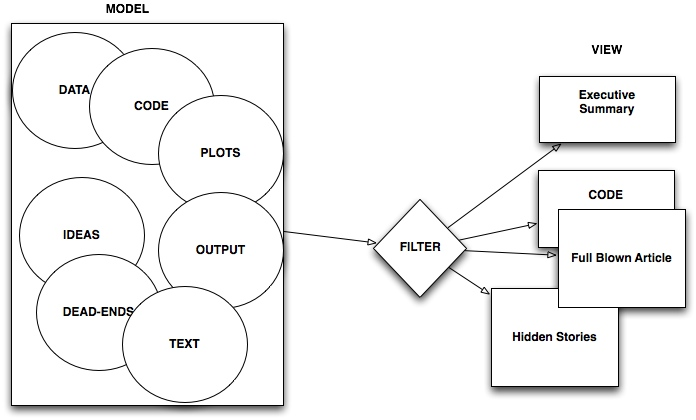
\includegraphics[width=4.5in]{images/DocumentDatabase.jpg}

\end{frame}

\begin{frame}[fragile] \frametitle{Structured Document}

\begin{itemize}
\item Handled programmatically
\item Rich Content - code, data, lab journal
\item Reproducible - recreate results
\item Reusable - extend, share
\item Intelligently searchable
\item Filtered for audience
\item Interactive - control parameters
\end{itemize}
\end{frame}  


\begin{frame}\frametitle{An Example: Geolocation}

\begin{itemize}
\item Inside a building, GPS do not provide an effective means 
for locating things. Instead, systems are built to use WiFi set up for Internet
access.

\medskip
  
\item In a lab setting,  received signal strength decays linearly with the log of
distance from the access point. 

\medskip
  
\item Walls, elevators, and people add noise to the received signal
strength. 

\medskip
  
\item Statistics can be helpful in developing a model to predict
location from the received signal strengths at other locations.

\end{itemize}
\end{frame}


%\begin{frame}\frametitle{Alternative analyses}
%\begin{itemize}
%\item Krishnan et al,\\
% A System for LEASE: Location Estimation Assisted by Stationery Emitters
%    for Indoor RF Wireless Networks (2004)
  
%\item King et al,\\
%COMPASS: A probabilistic indoor positioning system based on 802.11 and digital compasses, 

%\textit{Proceedings of the 1st international workshop on Wireless
 %     network testbeds, experimental evaluation \& characterization}, 

% (2006) 
  
%\item Youssef and Agrawala,\\
%On the Optimality of WLAN Location Determination Systems , 

%\textit{Proceedings of the Communication Networks and Distributed Systems  Modeling and Simulation Conference}, 

%(2004)
  
%\item Madigan et al,\\
%Location Estimation in Wireless Letworks: A Bayesian Approach,

%\textit{Statistica Sinica},    

%2006
%\end{itemize}
%\end{frame}

\begin{frame}\frametitle{Researcher's Analysis}
\begin{center}
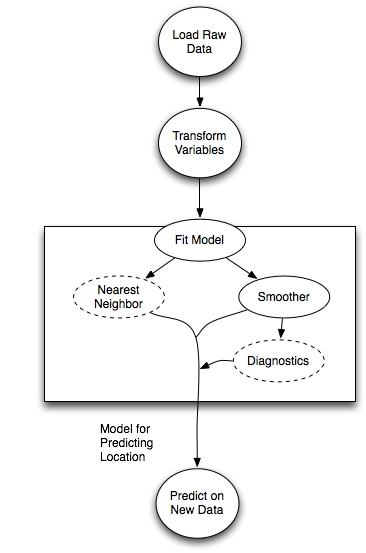
\includegraphics[width=2in]{images/WirelessDocumentDatabaseResearcher.jpg}
\end{center}
\end{frame}


\begin{frame}\frametitle{Instructor's Guide}
\begin{center}
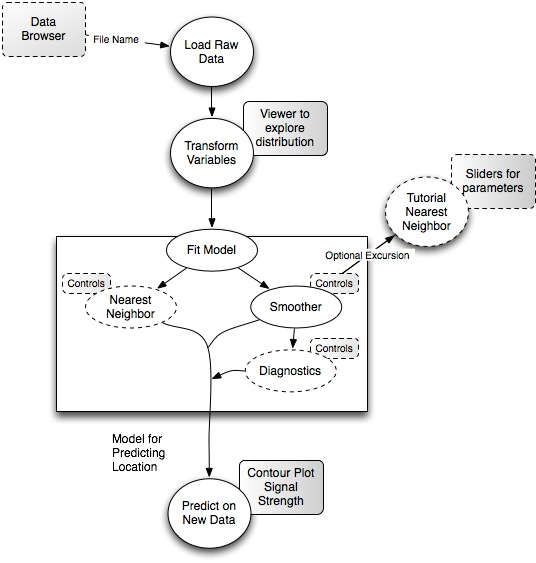
\includegraphics[width=3in]{images/WirelessDocumentDatabase.jpg}
\end{center}
\end{frame}


\begin{frame} \frametitle{Infrastructure - XML \& R}

\begin{block}{XML is not a markup language}
XML is a meta-language facility for defining a markup language. It provides a general framework for supplying meta-information to data. 
\end{block}

\begin{block}{}
\begin{columns}
 \begin{column}{0.45\textwidth}
 \begin{itemize}
  \item separates content from form
    \item human readable 
  \item easily generated by machine
 \end{itemize} 
\end{column}

  \begin{column}{0.45\textwidth}
 \begin{itemize}
   \item self-describing 
  \item extensible format
  \item strict parsing rules
  \item tools shared across disciplines
 \end{itemize} 
\end{column}
\end{columns}

\end{block}

\end{frame}


\begin{frame}[fragile]\frametitle{XML processing}
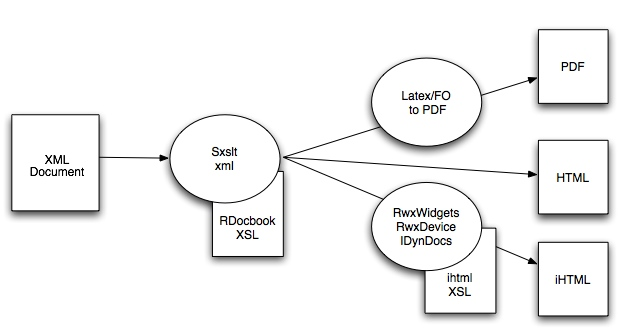
\includegraphics[width=4.5in]{images/XMLControlFlow.jpg}

\end{frame}

\begin{frame}[fragile] \frametitle{Future Directions}


\begin{itemize}
\item Foster community of contributors
\item Develop R plug-in for Firefox  
\end{itemize}
\end{frame}  


\end{document}
